\chapter{Measurement of Directional Characteristics III}\label{ax:directional_3}
This appendix serves as a protocol to a series of measurements conducted between the 10\textsuperscript{th} and 12\textsuperscript{th} of May  2018 in the large anechoic chamber (B4-111) at the acoustic lab of Aalborg University at Fredrik Bajers Vej 7.\\
The goal of these measurements is investigating the behaviour of a loudspeaker array consisting of three of the loudspeakers that have been featured in \autoref{ax:directional_1} and \ref{ax:directional_2}.

\section*{Measuring Equipment and Materials}
The following measuring equipment was used:
\begin{itemize}[noitemsep]
\item Microphone \gls{bandk} 4144
\begin{itemize}[noitemsep]
\item AAU-number: 06552
\item Serial number: 297090
\end{itemize}
\item Preamplifier GRAS 26AK
\begin{itemize}[noitemsep]
\item AAU-number: 56526
\item Serial number: 32810
\end{itemize}
\item Power supply \gls{bandk} 2636
\begin{itemize}
\item AAU-number: 08022
\item Serial number: 
\end{itemize}
\item Calibrator \gls{bandk}\ 4231
\begin{itemize}[noitemsep]
\item AAU-number: 33691
\item Serial number: 2115338
\end{itemize}
\item 2 pcs. Power Amplifier Pioneer A-616
\begin{itemize}[noitemsep]
\item AAU-number: 08249, 08699
\item Serial number: HJ9404841S, JG9405804S
\end{itemize}
\item Sound card RME Fireface UCX
\begin{itemize}[noitemsep]
\item AAU-number: 108230
\item Serial number: 23811948
\end{itemize}
\item Turntable: Outline ET 250-3D
\begin{itemize}
\item Serial number: REIB0012
\end{itemize}
\item MATLAB r2017b on OSX 10.11.6
\item 3 pcs. Loudspeaker SEAS 33 F-WKA
\end{itemize}

The following material was used:
\begin{itemize}[noitemsep]
%\item \SI{1/2}{\inch} to \SI{1}{\inch} preamp adapter
\item Microphone clip
\item Microphone stand
\item LEMU cable
\item \gls{bandk} cable
\item XLR cables
\item Ethernet cable
\item miscellanious adapters
\item 3 pcs. Loudspeaker cabinet, plywood, outside dimensions: (400x400x400)\SI{}{\milli\meter}, wall~thickness:~\SI{20}{\milli\meter}, equipped with \citep{seas33}
\item Speaker mount for turntable
\begin{itemize}[noitemsep]
\item Steel mounting contraption, see REFERENCE TO HARDWARE CHAPTER
\item 3 speaker legs, \SI{40}{\milli\meter} box section, top: aluminium, {\(\varnothing\)~:~\SI{34.8}{\milli\meter}}, height: \SI{1}{\meter}
\item Circular \gls{mdf} cutout, thickness: \SI{12}{\milli\meter}, {\(\varnothing\)~:~\SI{800}{\milli\meter}}
\item \gls{mdf} cutout, thickness: \SI{20}{\milli\meter}, surface: approx. (300x600)\SI{}{\milli\meter}, bolt pattern drilled according to the bottom side of the ET 250-3D turntable
\item \gls{mdf} cutout for counterweight mounting, thickness: \SI{12}{\milli\meter}, surface : (400x400)\SI{}{\milli\meter}
\item triangular cutout (isosceles), thickness: \SI{12}{\milli\meter}, approximate outside dimensions (base width x height): (970x600)\SI{}{\milli\meter}
\item 2 Electrovoice S-200 speakers as counterweight
\item Ratchet strap
\item 4 bolts M8x80, associated washers
\item 6 bolts M8x30, associated washers
\item 8 sinkhead bolts M8x40, associated nuts and washers
\item miscellaneous woodscrews

\end{itemize}
\end{itemize}



\section*{Setup}\label{sec:05_11_setup}
When setting up the speaker array according to dimensions that have been decided upon in \autoref{sec:opt_result}, a substential effort was undertaken to insure a secure stance. The turntable was mounted to one of the platform grids used in the anechoic chamber by screwing bolts through a \gls{mdf}-plate and the grid into the threads on the underside of the turntable. A round \gls{mdf} plate was mounted using the boltpattern on the upside of the turntable. Fixed to the round plate the custom made steel contraption (see \autoref{sec:hardware}) was bolted, which itself held the legs of the speakers in place. while allowing some adjustability. In a height of approx \SI{1}{\meter} above the turntable the three speaker cabinets were mounted to the legs. On top of the speaker a triangular \gls{mdf} cutout was employed to enhance rigidity. A picture of the array is given in \autoref{fig:05_11_setup}.

\begin{figure}[h]\label{fig:05_11_setup}
	\centering
    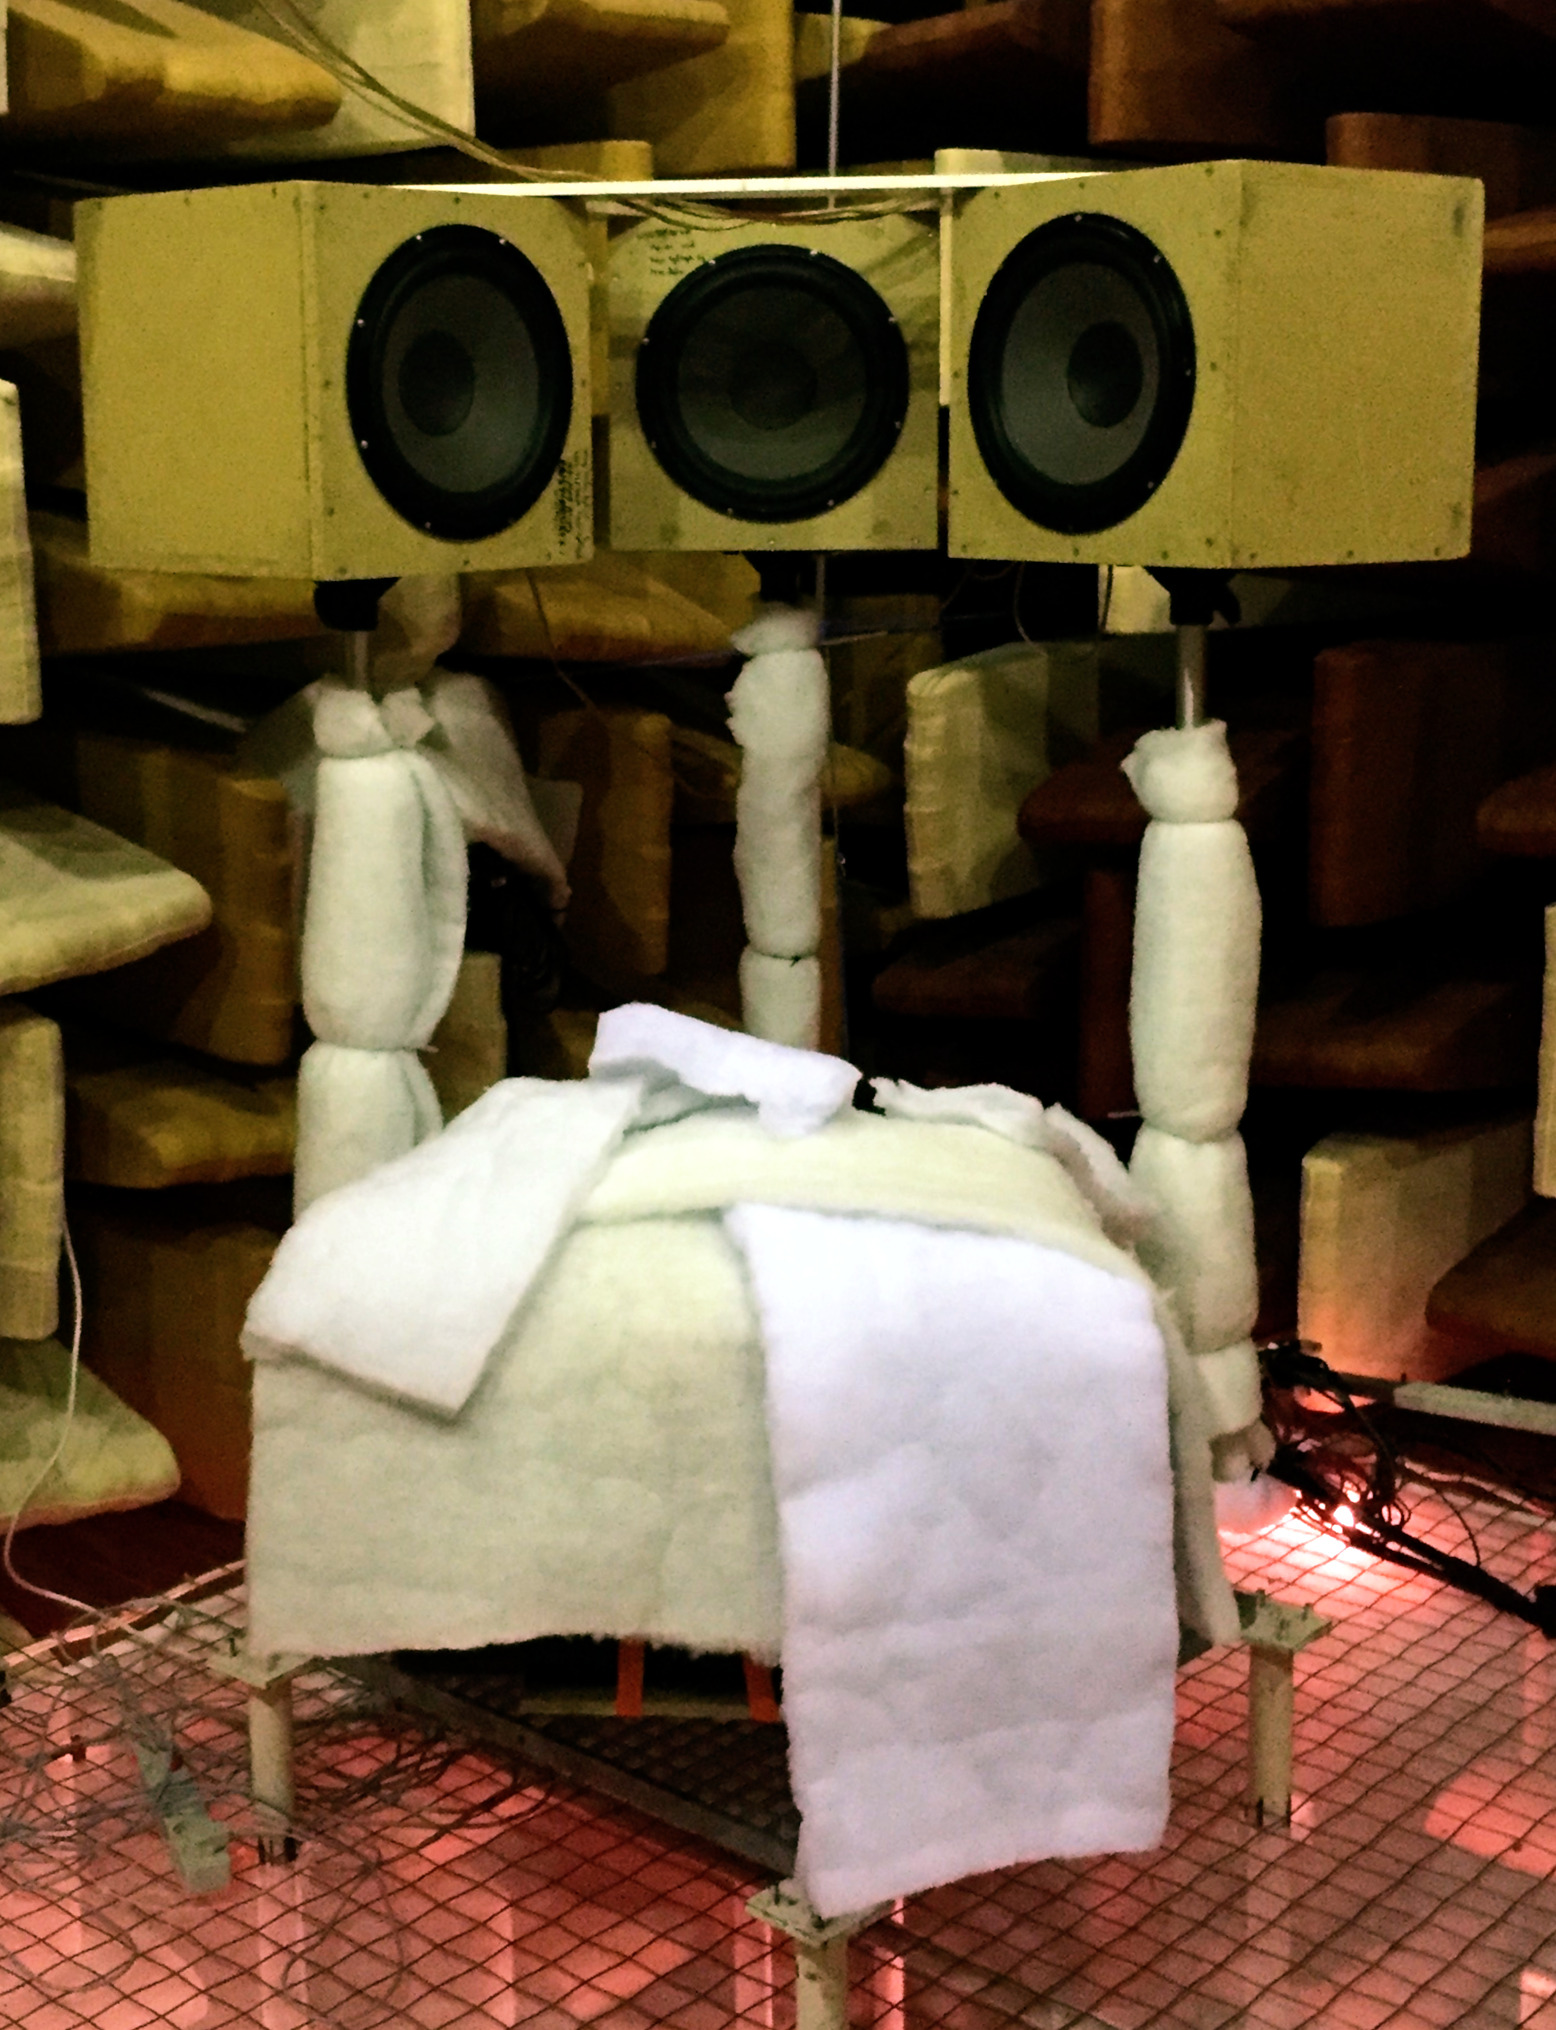
\includegraphics[width=0.5\textwidth]{05_11_setup.jpg}
    \caption{Speaker array setup on the turntable in the anechoic chamber.}
\end{figure}

The height of the centers of the speaker cabinet above the grid turned out to be \SI{1.37}{\meter}. The microphone was set up in the same height. Platforms for the speaker array and the microphone were set up in opposing corners of the anechoic chamber, which resulted in a horizontal distance between the array center and the microphone of \SI{4.92}{\meter}.
The input and the output gain of the \gls{bandk} 2636 microphone power supply were both set to \SI{+10}{\decibel}. The input gain on the Fireface UCX was set to \SI{0}{\decibel}. On the playback side, the power amplifiers had a fixed voltage gain of \SI{+10}{\decibel} and the \texttt{playgain}-parameter in the measurement routine was set to \SI{-10}{\decibel}. The playback signals were normed so that the absolute of the biggest amplitude in on of the filtered sweeps (see \autoref{sec:filter_design} is a digital value of 1.\\
The desired positioning of the acoustic centers of the speakers was found to be describable as \texttt{Lx}$\,=\,\SI{40}{\centi\meter}$ and \texttt{Ly}$\,=\,\SI{-40}{\centi\meter}$ in \autoref{sec:opt_result}. In order to make achieve the positioning without the loudspeaker cabinets physically interfering, the azimuth of both of the two front loudspeakers \texttt{B} and \texttt{C} was rotated by \SI{50}{\degree} inwards. The speaker positions were adjusted according to the finding of \autoref{ax:directional_2}, that the acoustic center of the speaker is approx. \SI{17}{\centi\meter}. The array center was set on the rotational axis of the turntable, in order to match the way, the point sources are set up in the analytical model and the \gls{fdtd} simulation.
This positioning was used as a baseline for measurements and was later adjusted to account for imprecisions and assymetries in the way the speakers were set up and further tweaked with an heuristic approach to changing the positions in order to achieve the best possible result with the given hardware and without changing the \gls{sp}-parameters. It is assumed that these tweeks were necessary in order to account for the influence that the speaker cabinets had on the sound field. By the time of the final measurements, the rear speaker \texttt{A} had been moved towards the front by \SI{4.5}{\centi\meter}, the side speakers had been moved towards the inside by \SI{2}{\centi\meter} each, and their azimuth angle had been increased to approx. \SI{55}{\degree}.
To illustrate the way, the speakers were set up, a birdseye view is given in \autoref{fig:array_pic}.
\begin{figure}[h]
	\centering
    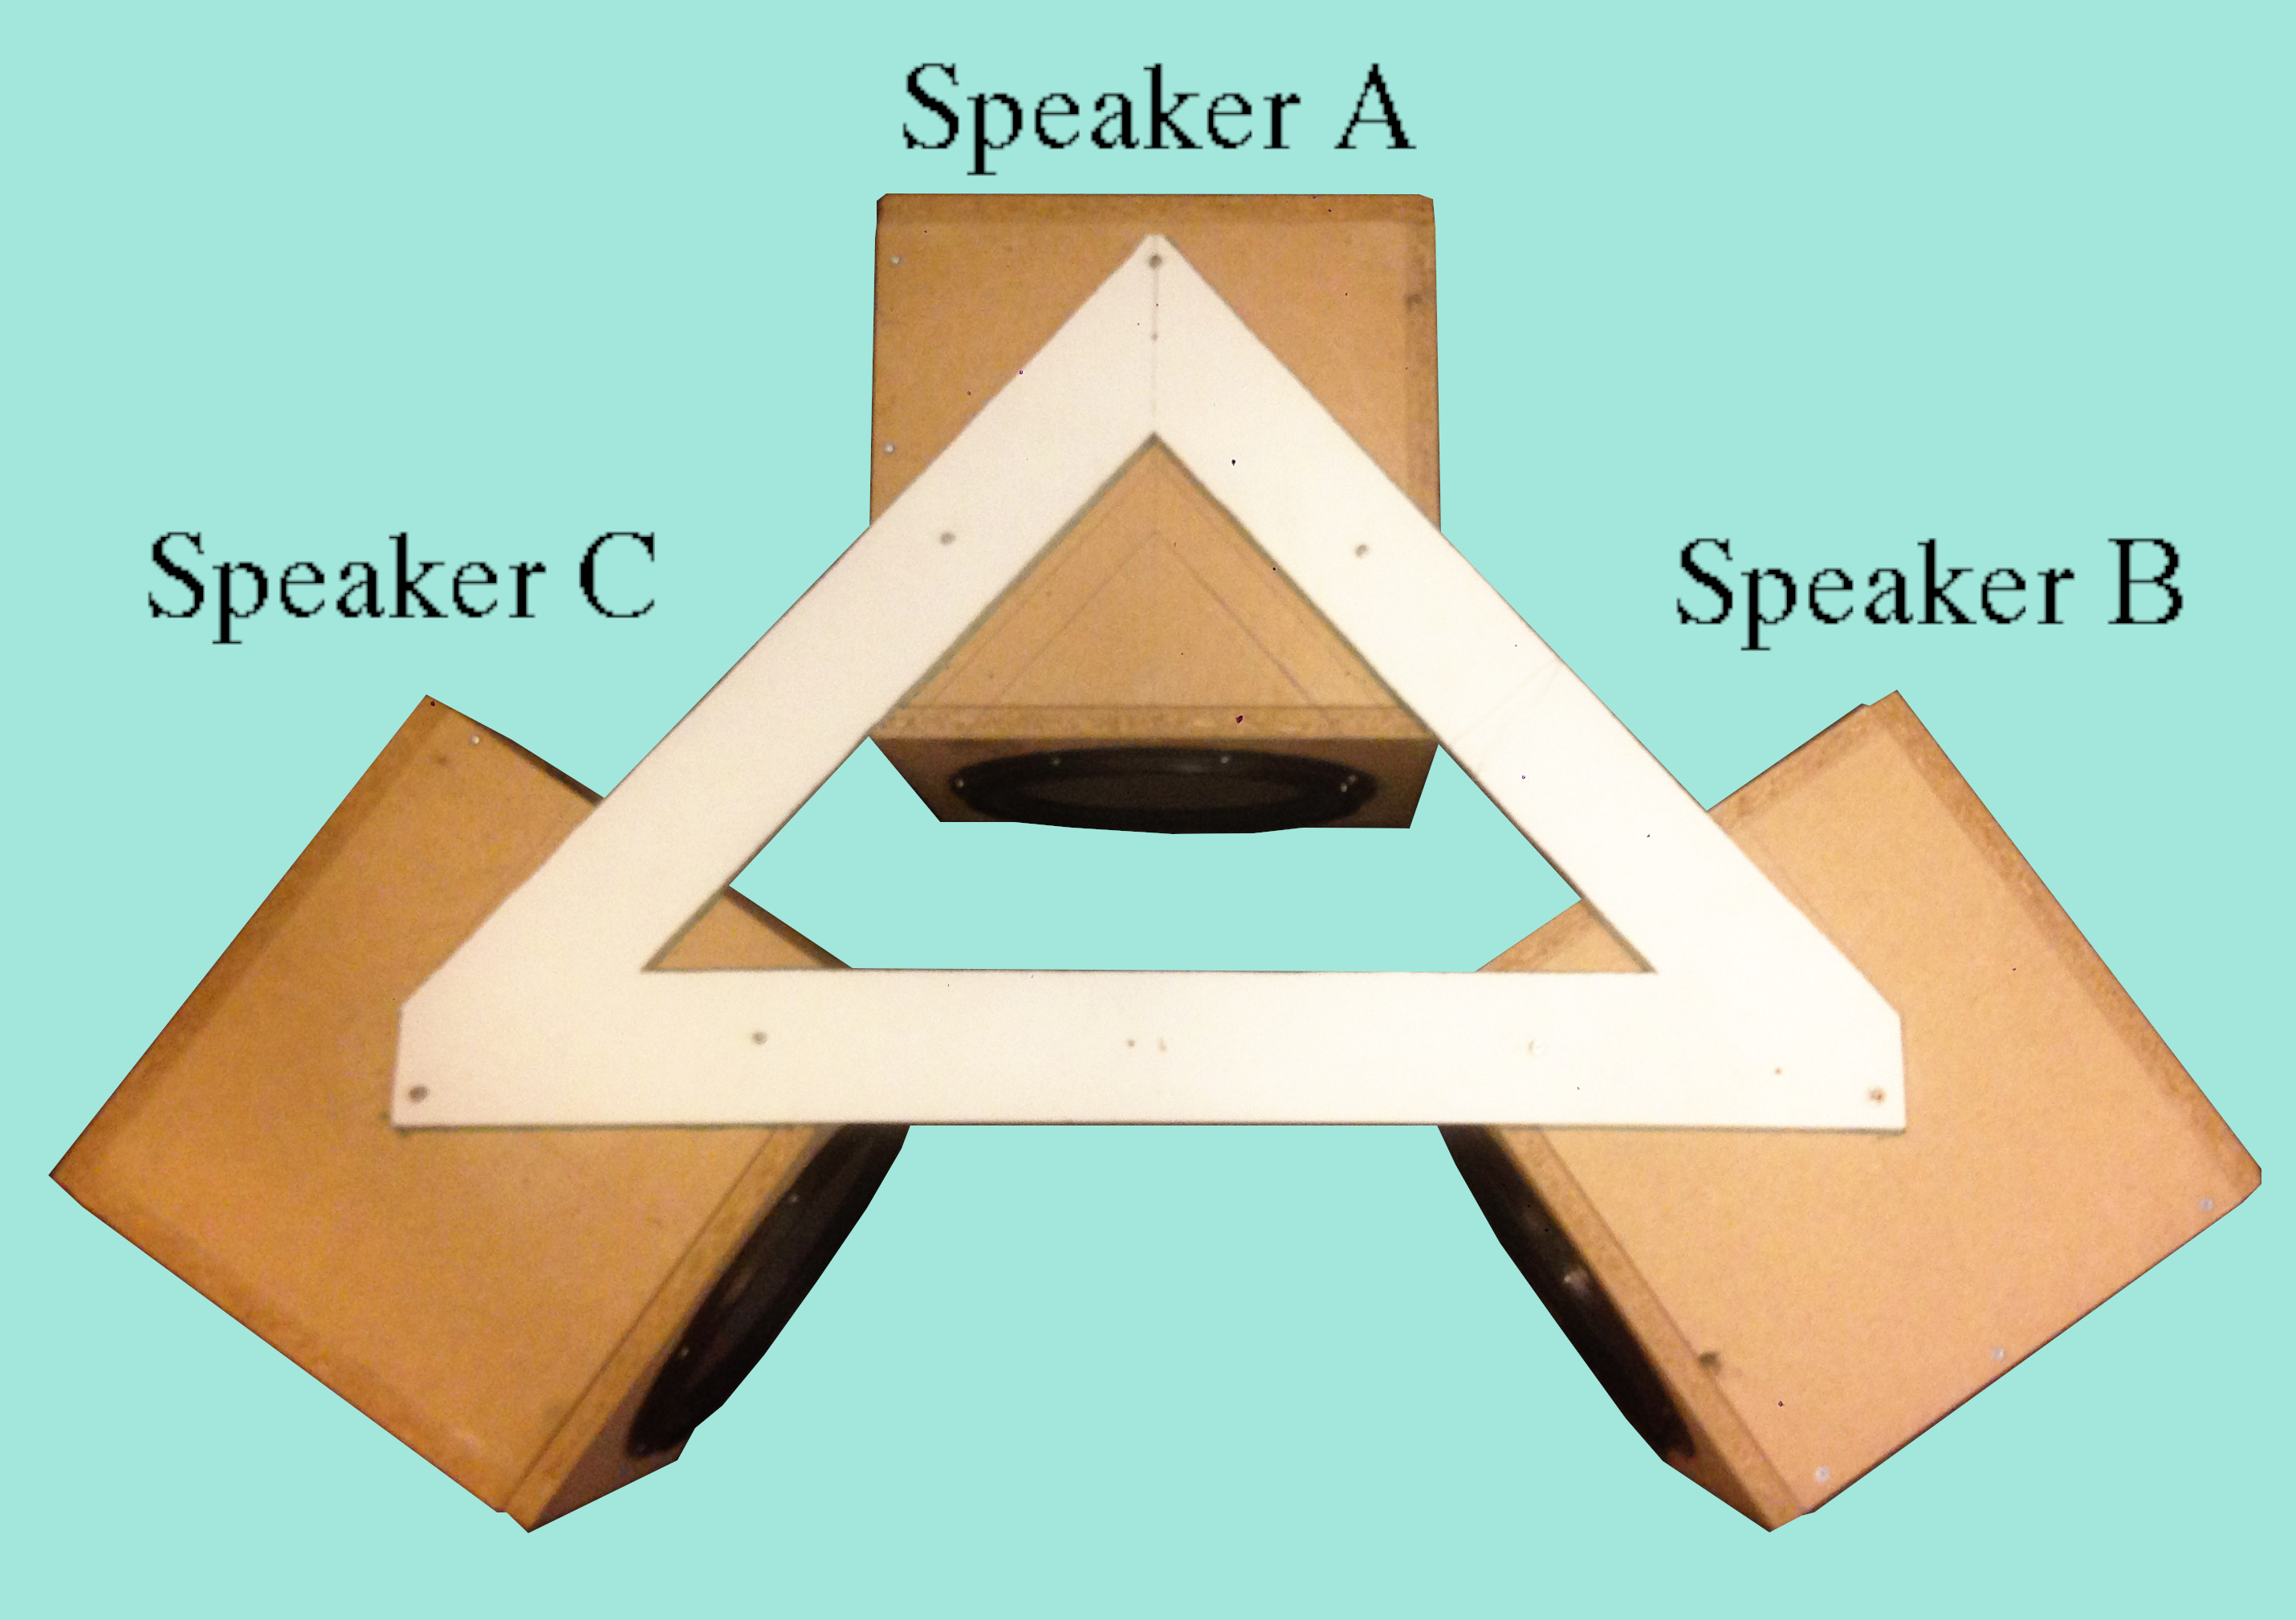
\includegraphics[width=0.5\textwidth]{speaker_array.jpg}
    \label{fig:array_pic}
    \caption{Speaker array arrangement}
\end{figure}

\section*{Results}\label{sec:05_11_results}
In the course of the measurement campaign, numerous polar responses have been measured. The main assessment on how the results are to be interpreted in the context of the overall project can be found in REFERENCE TO MAIN CHAPTER.\\
For this appendix, only an overview over the measured data is given.
The first measurement that was conducted, the polar response of the beamforming array with the speaker cabinets arranged in the inital positioning was recorded. The results are shown in \autoref{fig:05_11_initial}.
\begin{figure}[h]
\begin{subfigure}[c]{0.5\textwidth}
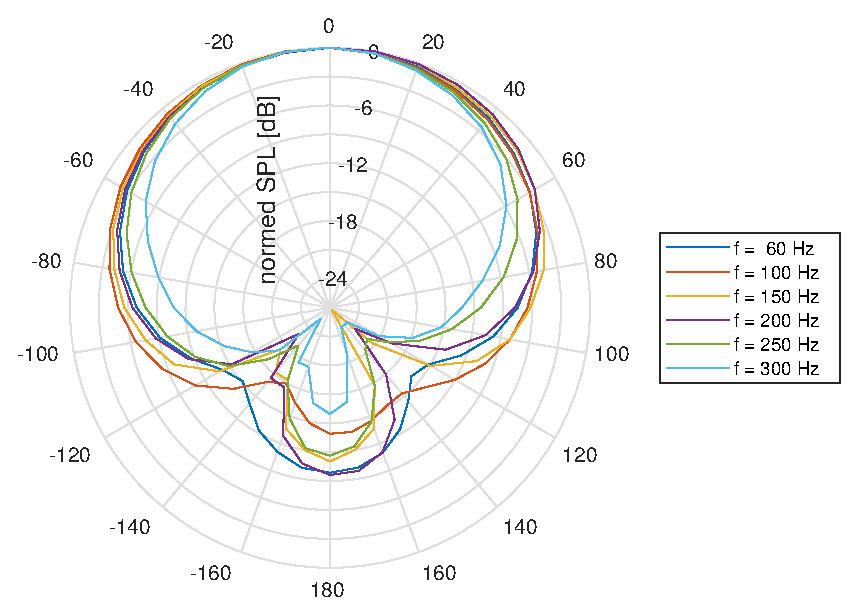
\includegraphics[width=0.85\textwidth]{05_11_initial_pr.eps}
\subcaption{Pressure}
\label{fig:05_11_init_pr}
\end{subfigure}
\begin{subfigure}[c]{0.5\textwidth}
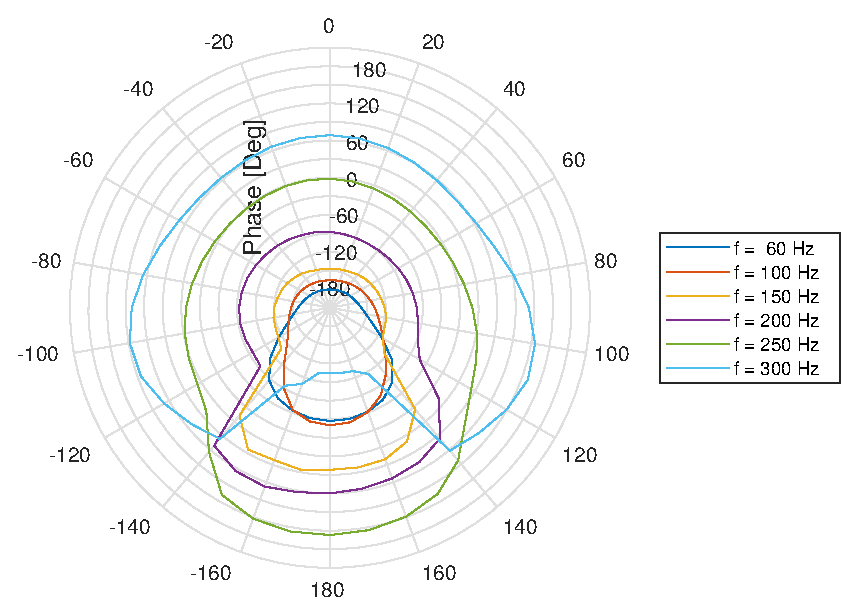
\includegraphics[width=0.95\textwidth]{05_11_initial_ph.eps}
\subcaption{Phase}
\label{fig:05_11_init_ph}
\end{subfigure}\\
\caption{Polar response, initial positioning}  
\label{fig:05_11_initial}
\end{figure}
Additional to verifying the beamforming capabilities of the array itself in combination with the chosen parameter set, the polar responses of each of the speakers has been measured, by disabling all signal processing that is related to the beamforming and disabling playback on the all but the measured speaker. The information gained in these measurements allows for verifying the symmetry of the setup as well as estimating the relative position of the acoustic in relation to the rotational axis of the turntable, which also is defined to be the array center. Also, more sophisticated pressure and phase correctional tables for the parameter optimization could be derived, if further development of the array is desired. The results are displayed in \autoref{fig:05_11_single}. These measurements were conducted with the speaker positioning, that had been adjusted as described in \autoref{sec:05_11_setup}.
The graphs can be compared with those displayed in \autoref{fig:03_02_m1_pressure} and \ref{fig:03_02_m1_phase}, which were measured with only a single speaker. The position of the speakers in the array is different in terms of distance of the acoustical center to the rotational axis of the turntable and the relation of the main axis of the speaker in terms of angle to the zero degree position of the turntable. If there was no significant influence of the speaker cabinets in the array on the directional characteristics of the individual speakers, all of the formerly mentioned graphs would only differ by a minimal shift of similar shapes in relation to the pole and in rotation. 
However, significant differences in the the shape of the graphs are apparent, e.g. when looking at \SI{250}{\hertz}-phase graphs. This indicates, that there is an influence of the speaker cabinets in the array on the way, sound emerges from the loudspeakers. The significance of this influence appears to be frequency dependent. The shape of the \SI{60}{\hertz} and \SI{100}{\hertz} graphs is close to circular in all of the measurements.

\begin{figure}[h]
\begin{subfigure}[c]{0.5\textwidth}
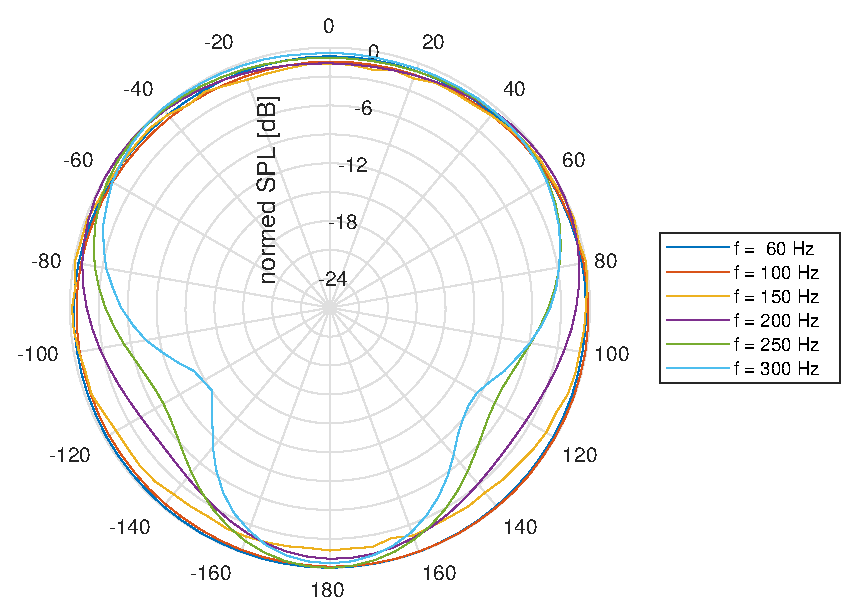
\includegraphics[width=0.85\textwidth]{05_11_A_pr.eps}
\subcaption{Speaker A, pressure}
\label{fig:05_11_A_pr}
\end{subfigure}
\begin{subfigure}[c]{0.5\textwidth}
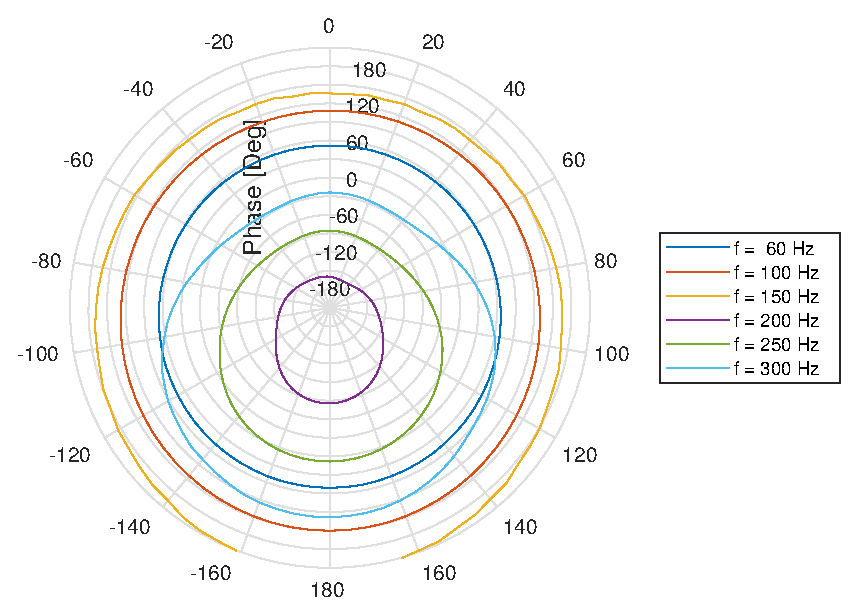
\includegraphics[width=0.95\textwidth]{05_11_A_ph.eps}
\subcaption{Speaker A, phase}
\label{fig:05_11_A_ph}
\end{subfigure}\\
\hspace{0.1\textheight}
\begin{subfigure}[c]{0.5\textwidth}
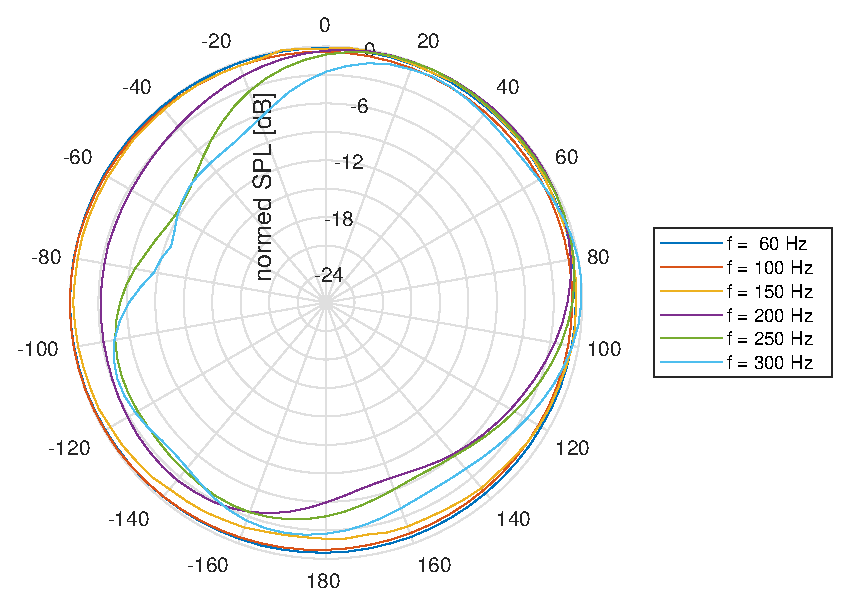
\includegraphics[width=0.85\textwidth]{05_11_B_pr.eps}
\subcaption{Speaker B, pressure}
\label{fig:05_11_A_pr}
\end{subfigure}
\begin{subfigure}[c]{0.5\textwidth}
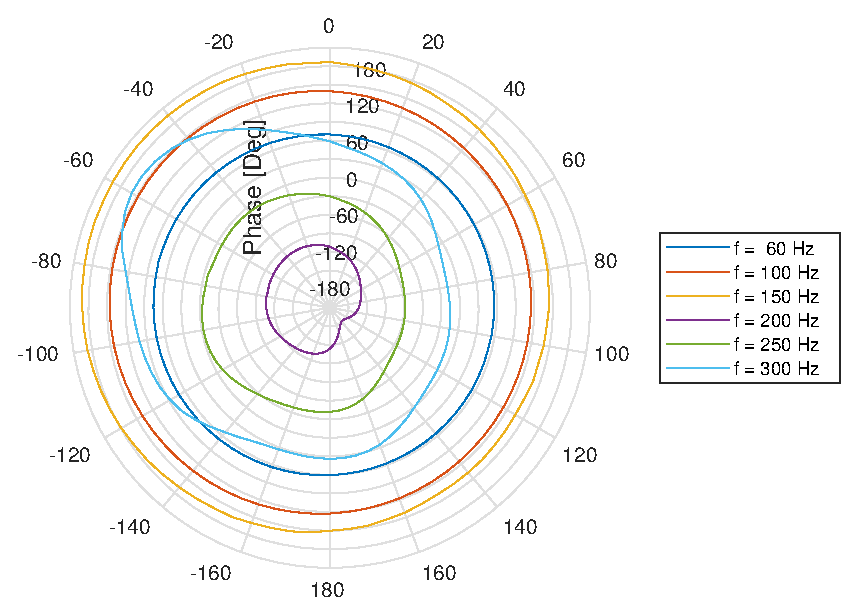
\includegraphics[width=0.95\textwidth]{05_11_B_ph.eps}
\subcaption{Speaker B, phase}
\label{fig:05_11_A_ph}
\end{subfigure}\\
\hspace{0.1\textheight}
\begin{subfigure}[c]{0.5\textwidth}
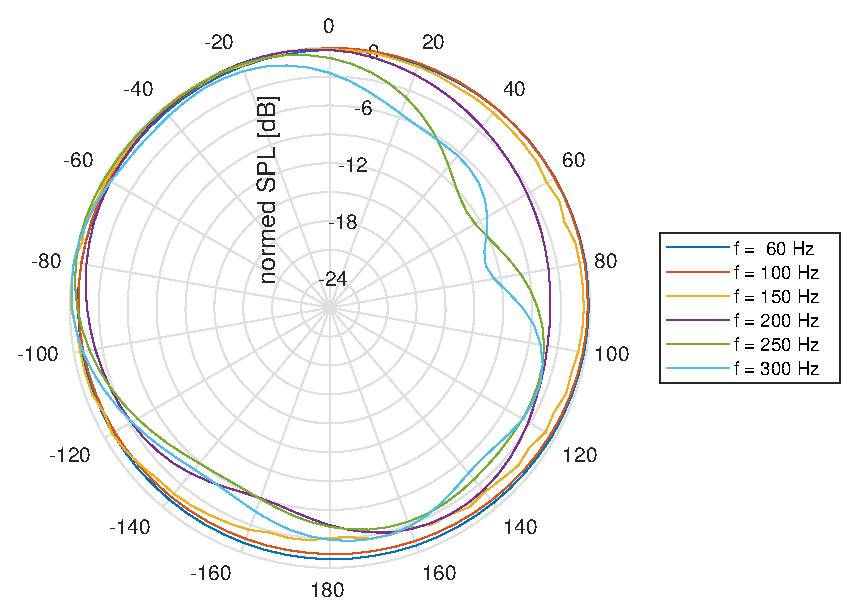
\includegraphics[width=0.85\textwidth]{05_11_C_pr.eps}
\subcaption{Speaker C, pressure}
\label{fig:05_11_A_pr}
\end{subfigure}
\begin{subfigure}[c]{0.5\textwidth}
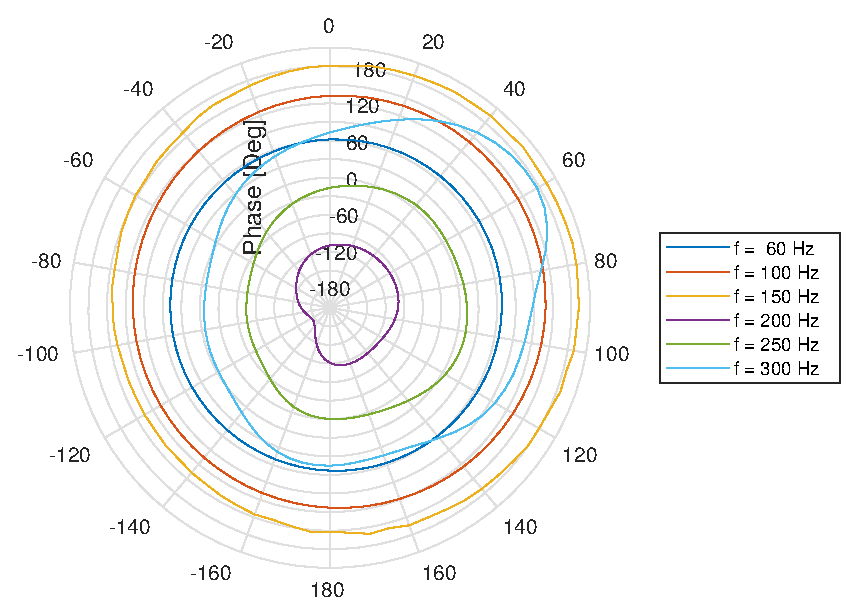
\includegraphics[width=0.95\textwidth]{05_11_C_ph.eps}
\subcaption{Speaker C, phase}
\label{fig:05_11_A_ph}
\end{subfigure}\\
\caption{Polar responses of each speakers alone, final positioning}  
\label{fig:05_11_single}
\end{figure}

Another measurement has been conducted, where all three speakers in the array played back the same signal. This means no beamforming was taking place. The results are displayed in \autoref{fig:05_11_all}. As well as serving as a baseline to how much attenuation is actually achieved by beamforming, this measurement can also provide a hint on weather the definition of the array center in \autoref{sec:genetic_implementation} has been a reasonable choice.
In \label{sec:ac_center}, the acoustic center has been established as the point in space, from which a virtual point source emitts sound. The conclusion from this is, that, when the acoustic center is placed on the rotational axis of the turntable during measurements, the resulting graphs in the polar plots of pressure and phase are circular and concentrical - just like the \SI{60}{\hertz} and \SI{100}{\hertz} pressure and phase graphs from the formerly mentioned measurement. 
Two things can be concluded from this. Firstly, placing the acoustic centers of a speaker array in a triangle leads to the centroid of this triangle acting as the acoustical center of the array, when all speakers play the same signal, which makes the decision to treat this position as the array center reasonable. Secondly, the adjustments, that have been made to the initial positions as described in \autoref{sec:05_11_setup}, have lead to positions of the acoustic centers, that are close to the desired positions.

\begin{figure}[h]
\begin{subfigure}[c]{0.5\textwidth}
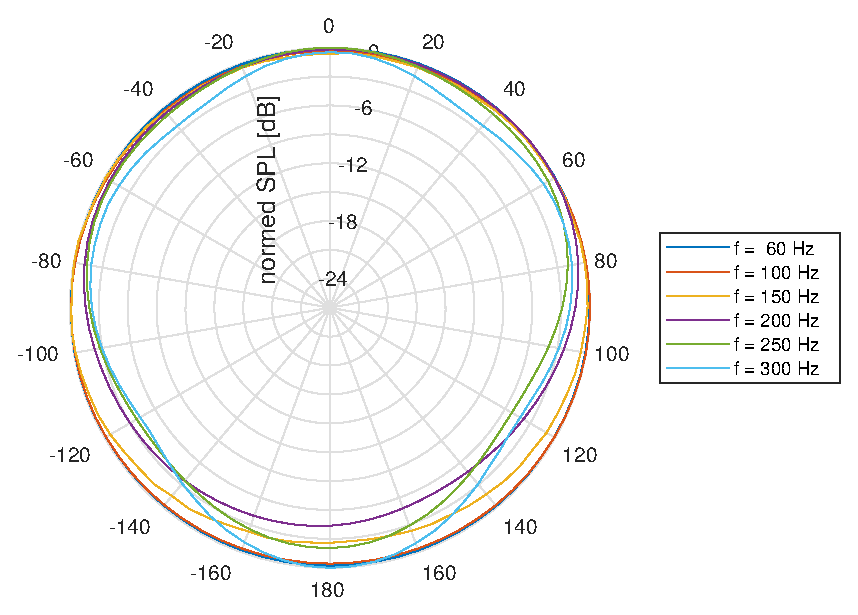
\includegraphics[width=0.85\textwidth]{05_11_all_pr.eps}
\subcaption{Pressure}
\label{fig:05_11_all_pr}
\end{subfigure}
\begin{subfigure}[c]{0.5\textwidth}
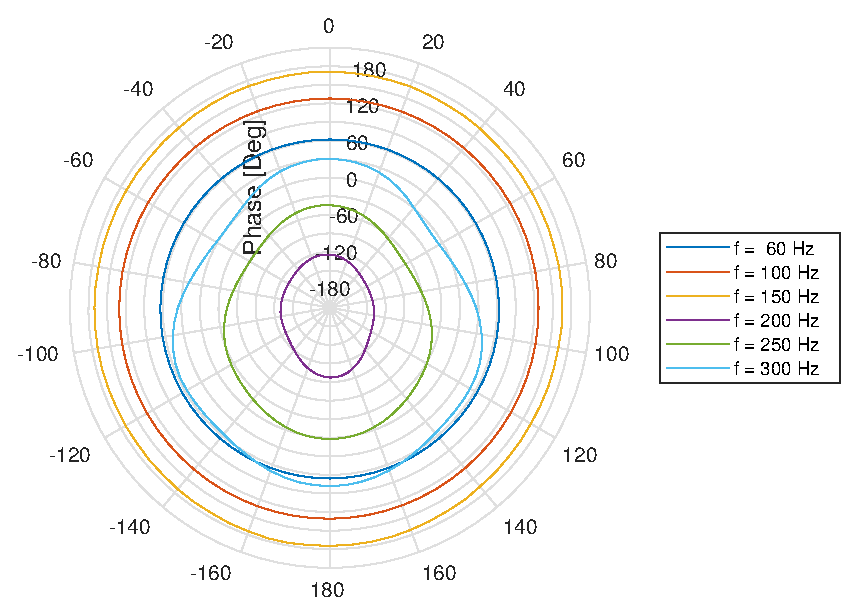
\includegraphics[width=0.95\textwidth]{05_11_all_ph.eps}
\subcaption{Phase}
\label{fig:05_11_all_ph}
\end{subfigure}\\
\caption{Polar response of the speaker array, beamforming disabled, final positioning}  
\label{fig:05_11_all}
\end{figure}

The directional characteristics of the speaker array with its final, adjusted positioning and the beamforming enabled by using filtering as described in \autoref{sec:filter_design} are shown in \autoref{fig:05_11_final}. A significant improvement over the characteristic with the inital positioning displayed in \autoref{fig:05_11_inital} has been achieved at the \SI{180}{\degree} direction. The attenuation compared to the main axis at this direction is bigger or equal to approx. \SI{12}{\decibel} at all frequencies. The maximum \SI{-3}{\decibel}-lobe width is approx. \SI{140}{\degree}, the maximum \SI{-3}{\decibel}-lobe width is approx. \SI{200}{\degree}. The phase graphs have a clearly non-circular shape. At roughly \SI{140}{\degree} and \SI{-140}{\degree} there are jumps in the phase graphs, between an approximately circular phase curve towards the main axis of the array and a phase shifted by anything between \SI{110}{\degree} and \SI{220}{\degree} compared to the front section.

\begin{figure}[h]
\begin{subfigure}[c]{0.5\textwidth}
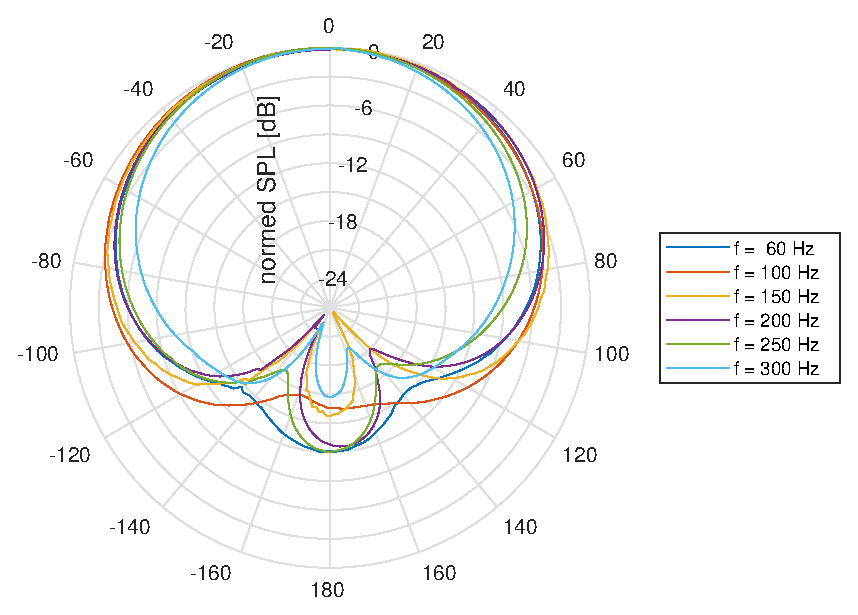
\includegraphics[width=0.85\textwidth]{05_11_final_pr.eps}
\subcaption{Pressure}
\label{fig:05_11_final_pr}
\end{subfigure}
\begin{subfigure}[c]{0.5\textwidth}
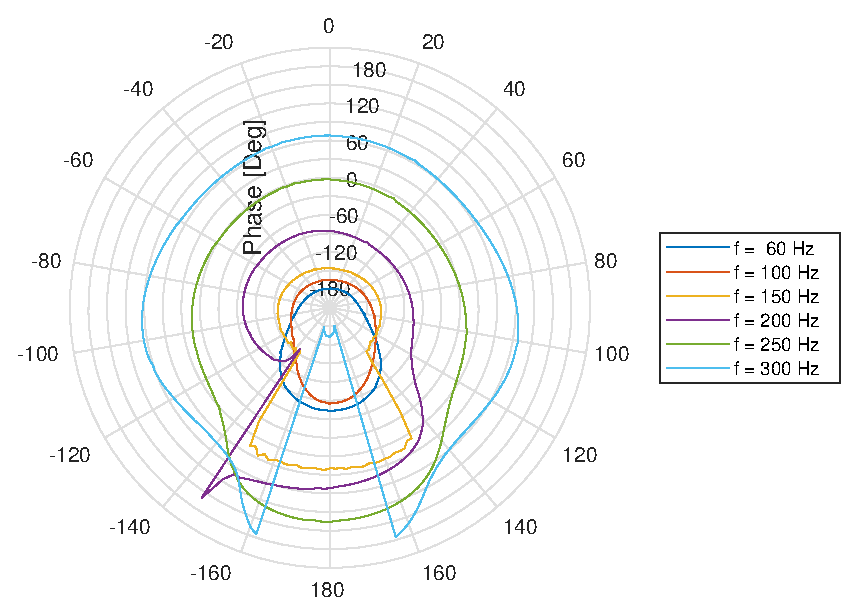
\includegraphics[width=0.95\textwidth]{05_11_final_ph.eps}
\subcaption{Phase}
\label{fig:05_11_final_ph}
\end{subfigure}\\
\caption{Polar response of the speaker array with beamforming, final positioning}  
\label{fig:05_11_final}
\end{figure}